% Select language used in document (ngerman or english). Automatically
% generated text is translated accordingly.
% use \selectthesislanguage in body.tex to switch to default language

%\documentclass[ngerman, paper]{mmt} % use for BA1
\documentclass[english, bachelorthesis]{mmt} % use for BA2
%\documentclass[ngerman, masterthesis]{mmt} % use for Master thesis

\usepackage{mathptmx}
\usepackage{graphicx}
\usepackage{times}
\usepackage{subfig}
\usepackage{float}
\usepackage[utf8]{inputenc}
\usepackage{listings}
\usepackage{makecell}
\usepackage[anythingbreaks]{breakurl}

% packages for tables
\usepackage{multirow}
\usepackage{booktabs}

\usepackage{amsmath}
\usepackage[autostyle,german=guillemets]{csquotes}

% moved to cls file. use \selectthesislanguage to switch to default language
%\usepackage[english,ngerman]{babel}

\usepackage{abbrevs}
%% the following solves a bug in the abbrevs package, that adds an empty
%% space after the abbrev
\makeatletter
\renewcommand\maybe@space@{%
  % \@tempswatrue % <= this is in the original
  \maybe@ictrue % <= this is new
  \expandafter   \@tfor
    \expandafter \reserved@a
    \expandafter :%
    \expandafter =%
                 \nospacelist
                 \do \t@st@ic
  % \if@tempswa % <= this is in the original
  \ifmaybe@ic % <= this is new
    \space
  \fi
}
\makeatother
%%


\usepackage{listings}
\usepackage{color}
\definecolor{lightgray}{rgb}{.9,.9,.9}
\definecolor{darkgray}{rgb}{.4,.4,.4}
\definecolor{purple}{rgb}{0.65, 0.12, 0.82}
\lstdefinelanguage{JavaScript}{
  keywords={break, case, catch, continue, debugger, default, delete, do, else, false, finally, for, function, if, in, instanceof, new, null, return, switch, this, throw, true, try, typeof, var, let, const, void, while, with},
  morecomment=[l]{//},
  morecomment=[s]{/*}{*/},
  morestring=[b]',
  morestring=[b]",
  ndkeywords={class, export, boolean, throw, implements, import, this},
  keywordstyle=\color{blue}\bfseries,
  ndkeywordstyle=\color{darkgray}\bfseries,
  identifierstyle=\color{black},
  commentstyle=\color{purple}\ttfamily,
  stringstyle=\color{red}\ttfamily,
  sensitive=true
}

\lstset{
   language=JavaScript,
   backgroundcolor=\color{lightgray},
   extendedchars=true,
   basicstyle=\footnotesize\ttfamily,
   showstringspaces=false,
   showspaces=false,
   numbers=left,
   numberstyle=\footnotesize,
   numbersep=9pt,
   tabsize=2,
   breaklines=true,
   showtabs=false,
   captionpos=b
}

\usepackage[authordate,bibencoding=auto,strict,noibid,backend=biber]{biblatex-chicago}
\bibliography{bibliography}

%% Add a list of acronyms
\usepackage{glossaries}
\makeglossaries
\newacronym{1nn}{1-NN}{nearest neighbor}
\newacronym{ann}{ANN}{artificial neural network}
\newacronym{ar}{AR}{Autoregressive}
\newacronym{api}{API}{application program interface}
\newacronym{csv}{CSV}{comma-separated values}
\newacronym{fft}{FFT}{fast Fourier transformation}
\newacronym{knn}{k-NN}{k-nearest neighbor}
\newacronym{rbf}{RBF}{radial basis function}
\newacronym{scut-naa}{SCUT-NAA}{South China University of Technology - Naturalistic 3D Acceleration-based Activity}
\newacronym{sma}{SMA}{signal magnitude area}
\newacronym{stft}{STFT}{short-time Fourier transform}
\newacronym{svm}{SVM}{support vector machine}

%% Add configuration options
\newabbrev{\authorname}{Alexander Moser}
\newabbrev{\authormail}{amoser.mmt-b2014@fh-salzburg.ac.at}
\newabbrev{\titlename}{Activity Recognition based on Generalized and Personalized Data Sets}
\newabbrev{\advisor}{FH-Prof. DI Dr. Simon Ginzinger, MSc}
\newabbrev{\thesisdate}{06.08.2018}
\newabbrev{\keywordsenglish}{Accelerometer, Activity Recognition, Support Vector Machine, Machine Learning, Feature Extraction}
\newabbrev{\keywordsgerman}{Beschleunigungssensor, wort2, wort3}


%% Paper title.

\title{\titlename}

%% This is how authors are specified in the conference style

%% Author 
\author{ \authorname\\ \scriptsize \authormail \\ \scriptsize 
\ifmmtlanguagegerman FH Salzburg \else Salzburg University of Applied Sciences \fi
}

%% A teaser figure can be included as follows, but is not recommended since
%% the space is now taken up by a full width abstract.
%\teaser{
%  \includegraphics[width=1.5in]{sample.eps}
%  \caption{This can be a teaser image of the thesis.}
%}

%% Abstract section for paper format.
\abstract{
    \ifmmtlanguagegerman 
        \selectlanguage{ngerman}
        % Kurzfassung

Diese Studie untersucht ein Datenset an Beschleunigungsdaten, um mit diesen unterschiedliche Lernalgorithmen zu trainieren. Diese sollen dadurch in der Lage sein, verschiedene Aktivitäten und Bewegungen voneinander unterscheiden zu können. Die Studie zeichnet sich vor allem dadurch aus, dass es möglich ist auch mit Daten ein Trainingsset zu erstellen, die unter natürlicheren Bedingungen als im Labor gesammelt wurden. Einerseits bedeutet dies, dass ein Accelerometer nicht unbedingt am Körper fixiert sein muss, sondern auch einfach lose in der Hosentasche platziert sein kann. Andererseits zeigt es auf, dass es nicht nötig ist, ein individuelles und personalisiertes Trainingsset für jede Testperson zu erstellen, um eine hohe Genauigkeit bei der Klassifizierung von Aktivitäten dieser Person zu erreichen.

Anfangs wurde versucht, die Daten über eine Webapplikation mit dem Smartphone aufzuzeichnen. Mehrere Personen führten verschiedene Aktivitäten aus, welche anschließend klassifiziert werden sollten. Da es dabei aber zu Problemen in der Auswertung kam, wurde ein zweiter Versuch gestartet, bei dem ein online zur Verfügung stehendes Datenset genutzt wurde.

Diese Studie beleuchtet dabei den Verlauf der Entwicklung beider Prototypen. Im Falle des ersten Versuches werden mögliche Gründe für die unzureichenden Ergebnisse genannt. Anhand des zweiten Versuchs wird erklärt, welche Schritte zu beachten sind, wenn man ein Datenset für einen Lernalgorithmus präparieren muss. Es werden verschiedene extrahierbare Features genannt und diese auf ihre Eignung zur Klassifizierung von Aktivitäten beurteilt. Weiters werden noch 3 verschiedene Lernalgorithmen untersucht und angewendet.
    \else 
        \selectlanguage{english}
        % Abstract

This paper examines a set of acceleration data, with the goal to train several machine learning algorithms. Thereby these algorithms should be able to differentiate between different activities and movements. This study highlights, that it is possible to create a generalized training set, even though the data was collected under a more naturalistic setting. On the one hand, this means that it is not necessary to fixate an accelerometer at the test subjects body, but it is sufficient to loosely place it in a trouser pocket. on the other hand this also means that it is not necessary to create a personalized training set for each individual to reach a high accuracy in activity recognition.

In the beginning the data was collected with a web application, using the accelerometer of a smart phone. Multiple people performed several activities, which were then classified. Since problems during the classification process occurred, the decision was made to start a new attempt with an online available data set.

This study highlights the progress of both prototypes. In case of the first prototype, this paper aims to provide reasons and explanations as to why these problems emerged, and how to avoid them in future applications. Based on the second attempt, this paper explains the necessary steps to process the raw acceleration data. It lists extractable features and judges their suitability for activity recognition. Finally it also takes a look at 3 different machine learning algorithms and their applicability.
    \fi
}

%%%%%%%%%%%%%%%%%%%%%%%%%%%%%%%%%%%%%%%%%%%%%%%%%%%%%%%%%%%%%%%%
%%%%%%%%%%%%%%%%%%%%%% START OF THE PAPER %%%%%%%%%%%%%%%%%%%%%%
%%%%%%%%%%%%%%%%%%%%%%%%%%%%%%%%%%%%%%%%%%%%%%%%%%%%%%%%%%%%%%%%%

\begin{document}

\selectthesislanguage

\pagenumbering{gobble}

 % group open
\ifmmtpaper 
\begingroup 
    % is required because paper template messes with sizes
    \fontsize{12}{18}\selectfont        
    \setlength{\parindent}{0pt}
    \setlength{\parskip}{5pt plus 2pt minus 1pt}
    \sectionfont{\fontsize{14}{15}\selectfont}
\fi

    \begin{titlepage}

% check if second advisor exists
\newcommand{\printsecondadvisor}[1]{%
  \ifcsname#1\endcsname%
  \ifmmtlanguagegerman ZweitbetreuerIn: \else Second Advisor: \fi \secondadvisor 
  \else%
    
  \fi%
}

\ifmmtmasterthesis

    
    % \begin{center}
    %     \Huge{ 
    %     	\textbf{\ifmmtlanguagegerman Masterarbeit \else Master Thesis \fi}
    %     }
    % \end{center}
    
    \newpage
    
    \thispagestyle{empty}
    
    \hfill 
\includegraphics[height=1.5cm]{images/FHSLogo.jpg}
    
    \vspace*{2cm}
    
    \Large{
    \titlename
    
    \vspace*{1cm}
    
    \ifmmtlanguagegerman
    Masterarbeit zur Erlangung des akademischen Grades
    \else
    Master thesis in partial fulfilment of the requirements for\\ the degree of 
    \fi
    
    \vspace*{0.5cm}
    
    \textit{Master of Science}
    }
    
    
    \vspace*{1.5cm}
    {\large
    \ifmmtlanguagegerman AuthorIn \else Author \fi: \authorname
    }
    \vfill
    
    {\normalsize
    \ifmmtlanguagegerman
    Vorgelegt am FH-Masterstudiengang MultiMediaTechnology, Fachhochschule Salzburg
    \else
    Submitted to the Master degree program MultiMediaTechnology, Salzburg University of Applied Sciences
    \fi
    
    
    \vspace*{1cm}
    
    \ifmmtlanguagegerman BetreuerIn: \else Advisor: \fi
    \advisor
    \\    
    \printsecondadvisor{secondadvisor}
    
    \vfill
    
    Salzburg, \ifmmtlanguagegerman Österreich, \else Austria, \fi  \thesisdate
    }

\else % Bachelor thesis title page

    \begin{center}
    
    
\includegraphics[width=5cm]{images/FHSLogo.jpg}


    \vspace*{4cm}
    
    \fontsize{20.79}{18pt}{\selectfont        
    %\Large{
    	\textit{\textbf{\titlename}}
    %}
    }
    
    \vspace*{4cm}
    
    \fontsize{20.79}{18pt}{%\large{
    \ifmmtlanguagegerman
    	\textbf{Bachelorarbeit \ifmmtpaper 1 \else 2 \fi }
    \else
        \textbf{Bachelor Thesis \ifmmtpaper 1 \else 2 \fi }
    \fi
    }
    
    
    \end{center}
    
    \vfill
    
    %\begin{tabular}{ll}
    \ifmmtlanguagegerman AuthorIn: \else Author: \fi  \authorname  \\
    \ifmmtlanguagegerman BetreuerIn: \else Advisor: \fi \advisor \\
    \printsecondadvisor{secondadvisor}
    
    Salzburg, \ifmmtlanguagegerman Österreich, \else Austria, \fi \thesisdate
    
    
    
    % uncomment the following 3 lines for an optional lock flag, max. 2 years!
    %\hfill
    %\color{red}
    %\framebox{Sperrvermerk bis 20/01/2012}

\fi

\end{titlepage}
        
    \onecolumn           
    
    \pagenumbering{roman}
    
    \newpage
    
\ifmmtlanguagegerman
\subsection*{Eidesstattliche Erklärung}


Ich erkläre hiermit eidesstattlich, dass ich die vorliegende Arbeit selbständig und ohne fremde Hilfe verfasst, und keine anderen als die angegeben Quellen und Hilfsmittel benutzt habe. Weiters versichere ich hiermit, dass ich die den benutzten Quellen wörtlich oder inhaltlich entnommenen Stellen als solche kenntlich gemacht habe.

Die Arbeit wurde bisher in gleicher oder ähnlicher Form keiner anderen Prüfungskommission weder im In- noch im Ausland vorgelegt und auch nicht veröffentlicht.

\else

\subsection*{Affidavit}

I herewith declare on oath that I wrote the present thesis without the help of third persons and without using any other sources and means listed herein; I further declare that I observed the guidelines for scientific work in the quotation of all unprinted sources, printed literature and phrases and concepts taken either word for word or according to meaning from the Internet and that I referenced all sources accordingly.

This thesis has not been submitted as an exam paper of identical or similar form, either in Austria or abroad and corresponds to the paper graded by the assessors.

\fi

\vspace*{3cm}

%{\bf \thesisdate{}}


\hfill

\ifmmtlanguagegerman
$\overline{Datum \hspace{2cm}}$ \hfill $\overline{{Unterschrift}\hspace{3cm}}$

\vspace*{1cm}

\hfill $\overline{{Vorname\hspace{2cm}Nachname}}$
 
 \else
 $\overline{Date \hspace{2cm}}$ \hfill $\overline{{Signature}\hspace{4cm}}$

\vspace*{1cm}

 \hfill $\overline{{First~Name\hspace{2cm}Last~Name}}$
 \fi

  % comment out for expose

% group closing
\ifmmtpaper
\endgroup
\fi

\ifmmtpaper\else
    
    \newpage
    \selectlanguage{ngerman}
    \section*{Kurzfassung}
    % Kurzfassung

Diese Studie untersucht ein Datenset an Beschleunigungsdaten, um mit diesen unterschiedliche Lernalgorithmen zu trainieren. Diese sollen dadurch in der Lage sein, verschiedene Aktivitäten und Bewegungen voneinander unterscheiden zu können. Die Studie zeichnet sich vor allem dadurch aus, dass es möglich ist auch mit Daten ein Trainingsset zu erstellen, die unter natürlicheren Bedingungen als im Labor gesammelt wurden. Einerseits bedeutet dies, dass ein Accelerometer nicht unbedingt am Körper fixiert sein muss, sondern auch einfach lose in der Hosentasche platziert sein kann. Andererseits zeigt es auf, dass es nicht nötig ist, ein individuelles und personalisiertes Trainingsset für jede Testperson zu erstellen, um eine hohe Genauigkeit bei der Klassifizierung von Aktivitäten dieser Person zu erreichen.

Anfangs wurde versucht, die Daten über eine Webapplikation mit dem Smartphone aufzuzeichnen. Mehrere Personen führten verschiedene Aktivitäten aus, welche anschließend klassifiziert werden sollten. Da es dabei aber zu Problemen in der Auswertung kam, wurde ein zweiter Versuch gestartet, bei dem ein online zur Verfügung stehendes Datenset genutzt wurde.

Diese Studie beleuchtet dabei den Verlauf der Entwicklung beider Prototypen. Im Falle des ersten Versuches werden mögliche Gründe für die unzureichenden Ergebnisse genannt. Anhand des zweiten Versuchs wird erklärt, welche Schritte zu beachten sind, wenn man ein Datenset für einen Lernalgorithmus präparieren muss. Es werden verschiedene extrahierbare Features genannt und diese auf ihre Eignung zur Klassifizierung von Aktivitäten beurteilt. Weiters werden noch 3 verschiedene Lernalgorithmen untersucht und angewendet.
    \ifmmtmasterthesis
    
    \vspace*{0.5cm} 
    \textbf{Schlüsselwörter:~} \keywordsgerman
    \fi
    \newpage
    \selectlanguage{english}
    \section*{Abstract}
    % Abstract

This paper examines a set of acceleration data, with the goal to train several machine learning algorithms. Thereby these algorithms should be able to differentiate between different activities and movements. This study highlights, that it is possible to create a generalized training set, even though the data was collected under a more naturalistic setting. On the one hand, this means that it is not necessary to fixate an accelerometer at the test subjects body, but it is sufficient to loosely place it in a trouser pocket. on the other hand this also means that it is not necessary to create a personalized training set for each individual to reach a high accuracy in activity recognition.

In the beginning the data was collected with a web application, using the accelerometer of a smart phone. Multiple people performed several activities, which were then classified. Since problems during the classification process occurred, the decision was made to start a new attempt with an online available data set.

This study highlights the progress of both prototypes. In case of the first prototype, this paper aims to provide reasons and explanations as to why these problems emerged, and how to avoid them in future applications. Based on the second attempt, this paper explains the necessary steps to process the raw acceleration data. It lists extractable features and judges their suitability for activity recognition. Finally it also takes a look at 3 different machine learning algorithms and their applicability.
    \ifmmtmasterthesis
        
    \vspace*{0.5cm} 
    \textbf{Keywords:~} \keywordsenglish
    \fi
    \selectthesislanguage
    
    \newpage
    \tableofcontents

\fi

\mmtcolumnmode % switch back to column formatting of stylesheet

\maketitle % used for paper formatting

\ifmmtpaper\else
\pagestyle{headings}
\fi
\pagenumbering{arabic}


%for reference to this section
\section{Introduction}
\label{section:introduction}

Activity recognition is a heavily researched topic, since its potential has yet to be fully utilized. If applied correctly it can support doctors from various medical fields, athletes during their training, or simply offer quality of life improvements for everyone.

Since mobile devices are a part of our everyday life, almost everyone carries an easily accessible accelerometer with them. They are equipped with versatile and sophisticated hardware. Their sensors are not only able to track GPS, direction and acceleration, but also audio, video, light, temperature and much more. Most important for the topic of this study is the data associated to the movement of the owner. These sensors are easy to read and provide the necessary data to analyze the activities and behavior of the user.

So the question arises, whether it is still necessary to collect movement data under clinical circumstances. Is it already possible to immediately get started by just downloading an application without the need to train it first? Typically when examining a patient they need to go through a series of tests, before being able to give an assessment. This takes a lot of time which both the user and the doctor must be willing to invest. In case of using a mobile application for personal use this can not be expected from people under normal circumstances. They are most likely not willing to invest the needed time, unless it is due to illness or other compelling situations.

A mobile application measuring the users data on the fly can be a significant improvement for physiotherapists. Their patients can just use their phone to recognize and classify their daily activities, instead of running tests for hours. This way more insight into the everyday life of the patient is offered, which allows for a profound diagnosis of certain conditions, like bone resorption. A general monitoring of exercises, including the usefulness of their effect, grant the physiotherapist more suitable assumptions about further treatment steps. 

Movement analysis can also be used as a preemptive measure. Elderly people become weaker until they reach the state of frailty, making them more prone to bone fractures, disorders and diseases. Therefore recognizing a decline in physical activity or a change in gait in time can help geriatrists to take counter measures against frailty early on and as a result to delay this development. Usually these precautions are based on the viewpoint of the geriatrist and physical tests outside of the patients accustomed environment. Having a tool to analyze their habits and activities can help the geriatrist greatly in giving a thorough diagnosis.

Medicine and health care are not the only fields of application though. Customizing the behaviour of our phone based on our current activity can work as a quality of life improvement. For example, if people go for a run, their phone could automatically switch to a non-disturbance mode, automatically redirecting calls to their voice mail. Fitness applications, or the phone by itself, could further use the collected data to evaluate whether the user is living healthy or not. Depending on the analysis, feedback regarding exercise recommendations could be given. 

Many studies provide ideas and strategies on how to approach activity recognition. Others offer an analysis of how accurate various machine learning algorithm can predict activities, or which features are best to be used. During the research for this paper barely any studies were found that used data which was gathered in a naturalistic setting. Most studies had a clinical setup, with acceleration sensors fixed to certain body parts, or running on a treadmill for example. Therefore this paper aims to answer the following questions.


\subsection{Research Intend}
First of all, is it possible to accomplish high accuracy of activity recognition when using data which is not collected under supervision in a clinical environment? Or is it sufficient to use loosely fixated accelerometer, like a mobile phone in a trouser pocket? Second, can a high enough classification probability\footnote{The accuracy describing, how often the correct classification is chosen} be reached when the gathered data of a test person is compared to movement data of other training subjects? Is it possible to predict activities and behavior, when the data is not compared to a personalized set of training data, but a generalized set consisting of many training subjects?

In both cases the expectation is that the accuracy will be lower. The main question is by how much. If it is not by a significant margin, the result could still have its own merits, favoring a vastly lower time investment at the cost of prediction accuracy. If this kind of activity recognition is successful, patients would not need to train an machine, but could instead immediately start with the analysis. This way more data could be gathered, especially with the possible development of future applications which incorporate this technology.

This study examines the accuracy of activity recognition when using data gathered under natural circumstances. The data is analyzed whether it is possible to create a generalized data set, which can be used for activity classification. It will try to answer, if it is still necessary to build up a new personalized training set for every user. This study takes a look at various machine learning algorithms, which features are best suited for classification and which activities are easiest to be recognized and differentiated. During the experiment a generalized data set will be created with the aim to classify activities of test subjects who are not part of said data set.


\subsection{Definitions}
In order to understand detailed results of the experiment the main objective needs to be defined beforehand. So the understanding of activity recognition in the context of this paper shall be explained.

Activity recognition or activity classification refers to the analysis and prediction of movement behaviors and patterns. An activity is a continuous and repetitive form of movement, like walking, running or climbing stairs. Every change in acceleration, rotation, shock and others, caused by certain movements are descriptive attributes of an activity. These descriptive elements are called features and are used for activity classification.

Further the understanding of a generalized and a personalized data set will be outlined. A data set refers to the collected data from the accelerometer. It contains the raw acceleration data for certain activities. A personalized data set contains the acceleration data of one test subject for all activities he or she has performed. A generalized data set on the other hand contains the personalized data sets of multiple individuals, preferably with acceleration data for each activity of every single participant.

\section{Related Work}
\label{section:related}

During prior research it was conducted that the choice of the correct machine learning algorithm and methods for pre-processing data is very important and can yield results with significant differences from one another. Studies such as "Human Activity Recognition via an Accelerometer-Enabled-Smartphone Using Kernel Discriminant Analysis" by \textcite[]{khan2010human}, as well as the paper "Activity Recognition using Cell Phone Accelerometers" by \textcite[]{kwapisz2011activity} achieved an activity recognition rate of up to 90\%. Another paper underlining this result is "Activity Recognition on an Accelerometer Embedded Mobile Phone with Varying Positions and Orientations" by \textcite[]{sun2010activity}. While all three delivered solid results, \textcite[]{kwapisz2011activity} fails to identify climbing stairs. The method of \textcite[]{khan2010human} using an \gls{ann} appears slightly superior to the \gls{svm} \textcite[]{sun2010activity} uses in terms of accuracy. However, an \gls{ann} and a \gls{svm} are both solid classification algorithms to choose for activity recognition in combination with the correct setup and enough training material.

Another noteworthy paper is "A Feature Extraction Method for Realtime Human Activity Recognition on Cell Phones" by \textcite[]{khan2011feature}. The researches from respectively the North South University in Dhaka (Bangladesh), the Marquette University in Milwaukee (USA) and the University of Wisconsin-Milwaukee in Milwaukee (USA) used a standard acceleration-based activity recognition data set, called \gls{scut-naa}, for extracting features from acceleration sensor signals. This allowed them to identify human activities, with which they hoped to contribute a novel linear-time method. The study revealed, that personalized training and testing data appears to be more useful than generalized data sets. Both of their methods brought them to the same conclusion. In this sense whether a \gls{svm} classifier with a linear kernel or with a \gls{rbf} kernel is applied, the level of accuracy remains the same.

The detailed researches ensured a knowledge base which helped to decide which technology is needed, to define the usefulness of the experiment itself as well as to estimate the expected outcome. The topics relevance in combination with the current technological developments ensure a positive outlook for the usage of activity recognition. From the throughout researched theoretical standpoint the practical part could be well structured. 


\subsection{Data Collection}
First of all the acceleration data from various test subjects needs to be gathered. A sophisticated data set is important, since it is the foundation of any test environment. \textcite[]{khan2011feature} for example used the \gls{scut-naa} data set. \textcite[]{xue2010naturalistic} created the data set by placing multiple sensors on the persons body and collecting the acceleration data via Bluetooth.

Alternatively a new set of data can be created, if the research team has new ideas on how to collect the data. In their study \textcite[]{kwapisz2011activity} used the accelerometer of a mobile phone to track the movement and acceleration of their test subjects.

Many studies performed the data collection on their own, but many also used preexisting data to save time and focus on their research question. If the way the data is collected is not important, then it is perfectly fine to use one that has been created by someone else. That is the reason why the \gls{scut-naa} data set is used in this study as well.

The previously mentioned studies collected various different activities. The most common of them were running, walking, climbing up or down the stairs, and resting. A test group was asked to perform these activities to collect the data and create personalized feature sets. Afterwards the data was analyzed and collectively evaluated. That way personalized sets of data for each individual were accessed, as well as an excessive set with the combined data was generated.

In the second part of the experiment the test group performed similar tasks as in the first part. The combined and personalized feature set were used to predict the activities of the test person. Additionally there were people in the second part of this test, which were not part of the learning process. This allowed for a fresh look at how well activities of people, who were not part of the first test group, can be recognized. To mimic this effect, this study will not train the classification algorithm with every test subject, but instead leave a few for testing.


\subsection{Data Processing}
There are different methods of reading and interpreting the signal from the accelerometer. For example the tilt of the device can be ignored, if you are only interested in the acceleration relative to its origin \autocite[]{kwapisz2011activity}. On the other hand, the tilt can also be used to estimate where the device is placed, if it is in the users hand, or in the users pocket \autocite[]{khan2011feature}. Another variable is the time window of how much data you should combine into one sample. While a 10-second segment might be sufficient to recognize long and repetitive movements like running or walking \autocite[]{kwapisz2011activity}, shorter activities might not be recognized, like climbing stairs.

After the pre-processing is completed, various features are calculated. \textcite[]{khan2010human} used \gls{ar} coefficients and the \gls{sma} to create feature vectors. Others like \textcite[]{kwapisz2011activity} used the average acceleration on each of the three axis, the standard deviation, the time between peaks and other to describe the characteristics of a movement. A collection of these feature vectors are called feature set. These are used by the aforementioned studies to train their algorithms and to test them.

\subsection{Machine Learning Algorithms}
The interpretation of the mobile data was done on a separated computer, which is powerful enough to handle performance intensive classification algorithms. A machine learning algorithm will be fed with the data in order to learn to distinguish between activities. The different studies found during the research process used a variety of different classification algorithms, including a decision tree, \gls{knn}, \gls{svm} and \gls{ann}. They also describe, how they configured them and how to avoid certain pitfalls.

\section{Classification Algorithms}
\label{section:classification}

To perform activity recognition, there are a variety of machine learning algorithms to consider. The ones used in this study are decision tree, k-nearest neighbor and support vector machine. This chapter aims to provide a detailed explanation for each of them.

All of the algorithms mentioned below are supervised learning models, meaning that they all need a set of input-output pairs. The input typically represents a vector of features, while the output represents the desired classification. This data is used to train the algorithm to generate a function which maps new feature vectors to one of the previously trained classes.


\subsection{Decision Tree}
A decision tree is a structure of nodes. Each node represents either a decision node, a chance node, or an end node. A decision node is a test on a property or feature, and branches off into two or more nodes. These again can be either of the three mentioned nodes. A chance node represents a decision which is based on probability, rather than being fully deterministic. An end node, or leaf node, is the last node of a branch and represents the outcome of the classification. A tree where every node branches off in only two nodes is called a binary decision tree. Every tree that has branches with more than two nodes can be converted into a binary decision tree.

In the case of activity recognition decision nodes represent the different features of each sample, like the magnitude of the acceleration, the direction of the acceleration along the three axes or the time between peaks. Each end node represents an activity the user can perform and which can be recognized, like walking, running or standing.

One of the benefits of decision trees is that they are quite easy to understand. After a short explanation, most people interpret a decision tree. In combination with an \gls{ann}\footnote{An \gls{ann} is a machine learning algorithm based on the idea of biological neural networks. It learns to perform tasks without prior knowledge, which also affect the structure of the \gls{ann}.}, it is possible to add new possible branches and outcomes, or just replace inefficient branches. This makes it suitable as a machine learning algorithm, since it can start developing its own branches and adjust already existing ones on its own.

Its main drawback is that they are relatively unstable, meaning that a decision tree might have to be heavily restructured when small changes to the data are made. This can mitigate a lot of prior work. Additionally they often tend to be quite inaccurate. Usually a decision tree yields worse results concerning accuracy and prediction, when compared to other classification algorithms. This is caused by its discrete decision making nature \autocite[]{king1995statlog, gascuel1998twelve}, as will be confirmed later in chapter \ref{section:results}. This gets alleviated by the fact that a decision tree can be combined with other machine learning algorithms. This way its performance can be improved and its accuracy can be increased. This is not investigated further during this study though.


\subsection{Nearest Neighbors}
The nearest neighbor algorithm is an algorithm which classifies data based on a nearest neighbor rule. When it is using the \gls{1nn} rule, the algorithm looks for the closest sample of a training set and will choose the same classification as the closest training sample it finds. In contrast the \gls{knn} rule does not only look for the closest training sample, but the K closest samples and chooses a classification based on a majority vote \autocite[]{cover1967nearest}.

There are different approaches for deciding which neighbors should be taken into consideration. The simplest and most straight forward way is to assign a class by majority decision. The more neighbors belong to the same class, the more likely it is, that the new sample belongs to the same class. Additionally a distance function could be implemented, giving neighbors which are closer to your sample more weight during the classification.

\begin{figure}[!ht]
    \centering
    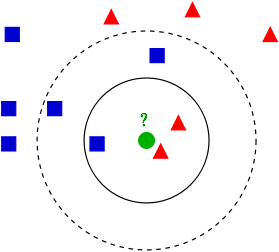
\includegraphics[width=0.5\linewidth]{images/Classification-Knn.png}
    \caption[]{
        K-Nearest Neighbor Classification \autocite[]{image-knn}
    }
    \label{figure:knn}
\end{figure}

It is oftentimes preferred to use \gls{knn} over \gls{1nn}. It takes more computational time, but especially in areas where samples tend to overlap and distinctions are not as clear, it improves the probability of a correct classification as it reduces the effect of noise \autocite[]{clusterAnalysis}. Therefore choosing a reasonable value for K is important. If K is too big, a lot of data has to be processed, and room for error is generated, since more neighbors of wrong classes could be taken into consideration. If K is too small though, noise may cause wrong classification as well. In figure \ref{figure:knn} a classification via \gls{1nn} would suggest that the green dot belongs to the class of red triangles. By using \gls{knn} with K = 5 the algorithm would determine that the green dot instead belongs to the blue squares. Which value is appropriate depends on the experiment and the desired outcome. As elaborated, this is an important part of the testing process.


\subsection{Support Vector Machine}
A previously mentioned, a \gls{svm} is a supervised learning model, which tries to find a hyper-plane\footnote{A hyper-plane is a geometrical subspace that has one less dimension than its ambient space. It separated the space into two half-spaces.}, that separates the different classes. The space between the samples of the training data and the hyper-plane has to be maximized. Depending on their position and distance relative to the hyper-plane new samples can be classified as either one of the two possible classes. This version of a \gls{svm} is called a Linear \gls{svm}. An example of this is shown in figure \ref{figure:svm}.

\begin{figure}[!ht]
    \centering
    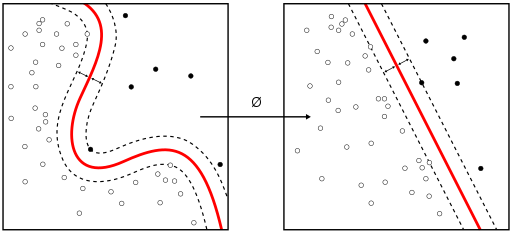
\includegraphics[width=0.75\linewidth]{images/Classification-Svm.png}
    \caption[]{
        Support Vector Machine Classification \autocite[]{image-svm}
    }
    \label{figure:svm}
\end{figure}

One upside of this algorithm is that not all training samples need to be considered for the generation of the hyper-plane. Samples which are surrounded by samples of the same class, or are further away from the plane, have no influence on the plane. This makes the computation a bit easier. The samples closest to the plane are stored as so-called support vectors, since they are sufficient to describe the hyper-plane.

A lot of times the sets of data are not linearly separable in their original space. This is often the case when there are more than two possible classifications. To approach a problem like this, kernel functions are used. These transform the data set into a higher dimensional space. At one point, if the number of dimensions is high enough, the data set will be linearly separable again by fitting a set of hyper-planes in this higher dimensional space \autocite[]{vert2004primer}.

Transformations like these are quite demanding, so transforming every sample into this higher dimensional space is not feasible. This is where the \textit{kernel trick} comes into play \autocite[]{vert2004primer}. By choosing the right kernel functions, the transformation becomes a lot easier. The effect of these kernel functions is that dot products can be computed very easily in both spaces, which equals the distance between the sample and the hyper-planes. This property is used to classify samples when using a \gls{svm}.

Examples of kernel functions for nonlinear \gls{svm} are a polynomial kernel and \gls{rbf}. These functions replace the dot product, when calculating the distance of each sample to the hyper-planes, with a function, that represents a distance function in a higher dimensional space \autocite{vert2004primer}.

A polynomial kernel (\ref{equation:polynomial-kernel}) can either be in-homogeneous or homogeneous if $c = 0$. The parameter $c$ is adding weight to either higher-order or lower-order terms in the polynomial.

\begin{equation}
    K_{poly}(\vec{x_{i}},\vec{x_{j}})=(\vec{x_{i}}\cdot\vec{x_{j}}+c)^{d}
    \label{equation:polynomial-kernel}
\end{equation}

An \gls{rbf} (\ref{equation:rbf-kernel}) is one of the most frequently used kernels in classification problems when using a \gls{svm}. It has a lot of favorable characteristics, like being able to generate non-parametric classification functions. Therefore almost any decision boundary can be obtained with this kernel. $\sigma$ is a parameter to tweak the kernel function. Smaller values lead to more complex decision boundaries, while larger ones will result in a smoother decision boundary \autocite{vert2004primer}.

\begin{equation}
    K_{rbf}(\vec{x_{i}},\vec{x_{j}})=\mathrm{exp}(-\frac{\left\|\vec{x_{i}}-\vec{x_{j}}\right\|^2}{2\sigma^{2}})
    \label{equation:rbf-kernel}
\end{equation}

While it is also possible to create and use custom kernel functions, it is not part of this study and will not be elaborated any further.

\section{Feature Extraction}
\label{section:features}

Since the raw data from the accelerometer can not be processed by the aforementioned classification algorithms, pre-processing the data is an important step of many classification processes. In this case the magnitude of the acceleration of every signal sample is calculated via the Pythagorean theorem. Since this results in losing any kind of directional indicators, the horizontal magnitude and vertical magnitude are calculated as well. This resulted in 3 variations of every feature, an absolute, a horizontal and a vertical version.

Several features can be generated from a subset of size $n$ of the magnitudes. These subsets are often overlapping in the hope that this will result in more similar features. This can also increase the accuracy of each individual feature, since it can be calculated from a bigger subset, while still maintaining the same number of features. Ultimately the aim is to be able to classify data well enough to grant reliable results. As previously mentioned the selection of features best suited for this process depends on the experiment and what kind of classification is sought. The ones that are used and examined in this study are the following:

\begin{itemize}
    \item Maximum amplitude
        
    \item Minimum amplitude

    \item Mean amplitude
        
    \item Standard Deviation
        
    \item Energy in time domain
        %\begin{equation}
        %    \mathrm{F}_{energy}=\sum_{i=1}^{n}x_{i}^{2}
        %\end{equation}
    
    \item Energy in frequency domain
    
    \item Hjorth Activity

    \item Hjorth Mobility

    \item Hjorth Complexity
\end{itemize}

In a given a window including $n$ samples $\{y(t), ..., y(t + n)\}$, the maximum will be the largest value, the minimum the smallest value and the mean amplitude will be the calculated average value $\bar{y}$ of these samples. The standard deviation represents the scattering of the samples from $\bar{y}$ and can be calculated via formula \ref{equation:standard-deviation}.

\begin{equation}
\label{equation:standard-deviation}
    \mathrm{Standard Deviation}=\sqrt{\frac{1}{n}\sum^{t}(y(t)-\bar{y})^{2}}
\end{equation}

The energy is calculated both in the time domain, as well as in the frequency domain. In the time domain, it equals the sum of the squared values of the sample window (\ref{equation:energy}). To get the energy transformed into frequency domain, a \gls{stft} has to be applied first to said sample window.

\begin{equation}
\label{equation:energy}
    \mathrm{Energy}=\sum^{t}y(t)^{2}
\end{equation}

The last three features are the so called Hjorth parameter and have been introduced by \textcite[]{hjorth1970eeg} in "EEG analysis based on time domain properties". The Hjorth Activity (\ref{equation:hjorth-activity}) hereby represents the signal power, the Hjorth Mobility (\ref{equation:hjorth-mobility}) represents the mean frequency and the Hjorth Complexity (\ref{equation:hjorth-complexity}) represents the change in frequency. They are calculated as follows:

\begin{equation}
\label{equation:hjorth-activity}
    \mathrm{Activity}=\mathrm{var}(y(t))
\end{equation}

\begin{equation}
\label{equation:hjorth-mobility}
    \mathrm{Mobility}=\sqrt{\frac{\mathrm{var}(\frac{\mathrm{d}y(t)}{\mathrm{d}t})}{\mathrm{var}(y(t))}}
\end{equation}

\begin{equation}
\label{equation:hjorth-complexity}
    \mathrm{Complexity}=\frac{\mathrm{Mobility}(\frac{\mathrm{d}y(t)}{\mathrm{d}t})}{\mathrm{Mobility}(y(t))}
\end{equation}

\section{Utilized Technologies}
\label{section:technologies}

The following chapter lists the technologies which were used to build the activity recognition application. It takes a closer look at them and describes them in detail for further understanding.

It took two iterations of building a prototype with different technologies before decent results could be obtained. The first attempt had to be discarded for reasons listed below. The second attempt yielded better results, which will be the main focus of the evaluation in chapter \ref{section:results} later on.

\subsection{First Approach}

The first attempt consists of two separate programs. They have very distinct responsibilities and can work independently from each other.

One is a web application used to collect the data from the accelerometer of a mobile phone. It is written in JavaScript, and perceives the phone's movement through listening to simple events. The collected data is then sent to an \gls{api} on a laptop in the same network to store said file.

The second program is built with Accord.NET \autocite[]{accord.net} and written in C\#. The Accord.Net framework is a machine learning framework, developed in C\# for scientific computing in .NET. It offers extensive libraries for signal, audio and video processing. Previous research conducted, that it is frequently used in scientific publications, which is one of the reasons why it is used in this study as well.

The program is designed to read multiple files created by the aforementioned web application and to classify the data. Each file represents an activity and while multiple files can represent the same activity, no file contains data of multiple activities. Various features, like energy, Hjorth mobility or Hjorth complexity, can be extracted from this data. The program then trains a \gls{svm} with the previously mentioned features. After the training is completed, it is capable to make predictions on data, which has not been used to train the algorithm before.

The results vary a lot when trying to predict activities. Sometimes this procedure does not yield any results at all. If the wrong combination of files are used to train the \gls{svm}, the training process will not terminate because it will keep trying to fit the data to a prediction model but is unable to do so. Once it finishes the training, the end results are reasonable when the algorithm was trying to predict activities from the same person. Trying to classify movement data of a person which has not been part of the training set led to a poor recognition rate. The accuracy of the prediction becomes incredibly low. On average the accuracy has been about 1/n where n is the number of possible activities.

There can be a multitude of reasons for this behavior. One could be that the data was not sufficient, because the frequency was too high, too low or the total time over which the activities were recorded was too short. Another reason could be that the cluster size of the data for calculating features was chosen too small. This was another consequence of the short recording time. A more detailed explanation will be elaborated in chapter \ref{section:results}. Ultimately it was decided to discard this attempt and build a new prototype with a different framework and an online available set of acceleration data.

\subsection{Second Approach}

The second attempt consists of only one program. It is a prototype written in Python and built with the Scikit-learn framework \autocite[]{scikit-learn}. This framework is an open source project that provides tools for data mining, data analysis and machine learning. It is heavily built on NumPy \autocite[]{NumPy} and SciPy \autocite[]{SciPy}, two powerful libraries for scientific computing with strong mathematical tools in Python.

This time the program focuses solely on feature extraction and classification algorithms. It reads acceleration samples from files and extracts various different features from them and then uses these to train machine learning algorithms like a decision tree, \gls{knn} or \gls{svm}. These are used to classify data sets, which were not used to train the algorithms, just like in the previous version.

The main difference between the two versions, besides the programming language, is the data set. In contrast to the first iteration, which collects the data through a mobile application, the second one uses an already existing data set called \gls{scut-naa}. The goal when creating this data set was to provide a sophisticated set of acceleration data, since at the time there was no comparable data set publicly available \autocite[]{xue2010naturalistic}.

\textcite[]{xue2010naturalistic} have aimed to produce a more naturalistic set of data. Most studies they looked at worked with data collected in a laboratory. Although these studies have had a high recognition rate, it dropped dramatically when providing the classification algorithm with data from a more naturalistic setting. \textcite[]{foerster1999detection} reported a classification accuracy of up to 95.8\%, which dropped to 66.7\% for data which has not been collected inside a laboratory.

It is a sophisticated data set, which also forms the basis of many other studies like the study "Assessment of Homomorphic Analysis for Human Activity Recognition From Acceleration Signals" of \textcite[]{vanrell2017assessment}. A more detailed description of how the data for \gls{scut-naa} has been gathered will be given in the following chapter.

\section{Experiment}
\label{section:experiment}
The focus of this chapter will be the execution of the two experiments. One experiment was focused on collecting acceleration data and then processing and classifying the resulting data sets. Since the second setup used a preexisting data set, its focus instead laid exclusively on the classification of activities.

\subsection{First Experiment}
As previously mentioned in the previous chapter the first prototype is split into two separated programs, each with their own individual tasks and challenges. The goal of the first program is to collect acceleration data and to store it, while the second part is trying to process that data. After extracting various features and training the machine learning algorithm, the second program should be able to classify new data as previously trained activities.

In the first round of gathering data, 5 test subjects were given a mobile phone, a Samsung Galaxy S6. On this phone they launched a web application. The application collected the acceleration data once the test subject started the recording. They had to select which activity they were going to perform and they had six different activities to choose from: walking, running, going upstairs, going downstairs, jumping and standing still. Each activity had to be performed multiple times for approximately 10 seconds each, resulting in a collection of about 4-8 files for each activity per person.

The application recorded acceleration samples at a frequency of 20 Hz and stored it locally on the mobile phone in a \gls{csv} file. Once the recording of an activity was completed, the file was sent to a laptop in the same network. Having to be in the same network made recording data difficult. Some activities, like running for example, were not possible to be performed for an extended period of time, since all tests had to be done indoors. Instead they had to be done in short succession of each other, each time stopping and restarting the recording of the acceleration.

After the collection of the data from one person was completed, the data files were transferred to the second program. This personalized data set was then processed to create feature files. It calculated the energy, Hjorth mobility and Hjorth complexity, each of these features separated into a horizontal and a vertical part. Therefore for further testing six features were available.

This process resulted in one feature file per person in the form of a \gls{csv} file. The structure of these files was set up to contain an integer as its first entry, which corresponds to the activity this row belongs to. The following entries of this row represent a feature vector for this activity.

After creating said feature files, the machine learning algorithms could be trained and tested. This first iteration of a prototype focused solely on using a \gls{svm} for classification. To train this algorithm, the features first needed to be scaled to look standard normally distributed, with a mean of 0 and unit variance. Without this step, the classification algorithm might behave unpredictable. A random collection of scaled features were then picked to train the \gls{svm}. Left out samples could then be used for cross validation and checking how successful the training was. In regard to the research question of this study, 4 feature sets of the 5 test subjects were used to train the \gls{svm}, while the 5$^{th}$ was being classified.

On a larger scale, this would be the approach to generate a generalized data set for activity recognition. First Collect the data of a larger group of training subjects, then train the classification algorithm on their movement patterns. Finally compare it to a new feature set of a test subject, which was not part of the training group.

As already mentioned in chapter \ref{section:technologies} the experiment utilizing the technologies mentioned here was not pursued any further, as too many problems occurred. The encountered issues will be explained in chapter \ref{section:results}.


\subsection{Second Experiment}
In chapter \ref{section:technologies} it was already mentioned that the second prototype utilizes the \gls{scut-naa} data set instead of gathering data itself. This data set contains the acceleration data of 44 test subjects (34 males and 10 females) each performing ten different activities. During their performance the data has been collected by three independent triaxial accelerometer at a frequency of 100Hz.

The three accelerometer have been placed in the subjects trouser pocket, at their waist and in their shirt pocket. Since the sensors have not been fixed to the body, they may have moved randomly in the pockets, which causes more variance in the data. This is not an undesirable effect though, since \textcite[]{xue2010naturalistic} have aimed to produce a more naturalistic set of data.

The next step is calculating the features. The second prototype implements all of the features mentioned in chapter \ref{section:features}: mean, maximum and minimum amplitude, standard deviation, energy in time as well as frequency domain and the 3 Hjorth parameter. All of these features get calculated from the absolute amplitude of the signal, its horizontal component and its vertical component, resulting in a feature vector with 27 different features. These get stored in a feature file, similar to how they have been stored during the first experiment. This saves time when using different combinations of features by not having to calculate them again every time.

Another factor that can have a big impact on the accuracy of the prediction is the cluster size from which the features are calculated. A feature calculated from a larger cluster contains more information about the activity, which will most likely increase to probability of a correct classification. On the downside, the feature set will end up with fewer feature vectors. Since we have less feature vectors to train the algorithm with, this could result in less accuracy. Therefore all features were calculated for 3 different sample sizes, 64, 256 and 512.

Since the goal is to find out which features are best used to train and test for activity recognition, various combinations of features need to be chosen. The prototype is built in a way to easily filter out unwanted features. They then get scaled to look normally distributed with a mean of 0 and unit variance again. The Scikit-learn framework implements a standard scaler, which gets fit to the training set. This scaler can then later be used to apply the same transformation to the test set.

The program does not only use one machine learning algorithm like the previous one to classify activities. It utilizes all of the ones explained in chapter \ref{section:classification}: decision tree, \gls{knn} and \gls{svm} with a linear kernel and \gls{svm} with a \gls{rbf} kernel. Chapter \ref{section:results} highlights the different results and aims to explain them.

\section{Results}
\label{section:results}
The following chapter is focusing on the results received from both experiments. The first experiment did not yield any reasonable results which is why chapter \ref{section:first-results} can not elaborate on such. Instead it will only look at possible reasons, why the experiment didn't work out the way it was supposed to. Afterwards chapter \ref{section:second-results} shows the results of the second prototype and explains different results based on different setups.




\subsection{Results of the First Prototype}
\label{section:first-results}
Most of the time the first prototype did not deliver high accuracy during classification. Sometimes it was not even able to start the classification process and the program never terminated. This was due to multiple reasons.

The first reason for the inconsistency was the data set. Since the experimental setup aimed to provide its own data set, this may be prone to be another source of errors. As already mentioned collecting data was tricky, since the participants of the study needed to stay within reach of the network of a laptop. After every completion of an activity, the mobile application sent the data directly to the laptop to store it. This resulted in very small data sets, since participants could not enact an activity over a long period of time. Especially an activity like running proved to be difficult to record. All activities needed to be performed inside which limited the available space.

To get enough data, either the sample frequency needed to be increased, or the participants needed to repeat each activity multiple times. Increasing the frequency seemed inadequate, since an activity could not be performed for longer than 5 to 10 seconds. So the goal was to get multiple recordings of the same activity instead of a higher resolution of one recording. In hindsight this was most likely a mistake. A sampling frequency of 20 Hz seems rather low, when compared to a frequency of 100 Hz as it was used by \textcite{xue2010naturalistic}.

This issue could have been avoided by making the application capable of working offline and synchronizing the data once the mobile phone was connected to the network again. This way activities could have been recorded over a longer period of time and without spatial restrictions. This challenge would have been approached first, if there had not also been a lot of problems during the classification process as well.

After collecting the acceleration data, it needed to be prepared properly, before features could be extracted from it. Since the participants needed to start and to stop the data recording manually, there is unwanted noise at the beginning and the end of such a data file. The test subject needed to put the mobile phone into their pocket and pull it out at the end, respectively. This noise needed to be filtered out, consequently reducing the amount of raw acceleration data per file even more. Because of that the data was even less consistent. Again, this could have been prevented by simply having longer recordings. Alternatively the process of recording could be started remotely by someone else other than the participant.

The next step was to calculate various features. The first prototype incorporated only 3 different features to begin with, the time domain energy, the Hjorth mobility and the Hjorth complexity. It was planned to add more features once the first few tests delivered some reasonable results, as was later the case with the second iteration of this experiment. Unfortunately this prototype had problems with the training of the \gls{svm}. When the training set consisted of features of only one participant and was then cross validated with data from the same person, the accuracy of the prediction was about 95\%. If the algorithm tried to predict the activities of another person, the accuracy dropped considerably. Taking a look at the resulting confusion matrix, it turns out that every possible outcome was equally likely to occur when trying to classify an unknown activity. Having trained the \gls{svm} on only 3 different activities, this means that there is only a 33\% chance of getting the correct prediction.

All of these problems led to the conclusion that restarting the experiment is probably better, than trying to fix these issues in the existing setup. By using a publicly available data set, the sources of error concerning the data set itself can be eliminated. It seems fair to assume that a data set, that is often used in scientific studies, is without major mistakes. As to not run into the same dead ends and pitfalls as before, the decision was made to also switch to a different framework. That is why Scikit-learn was used in the second iteration instead of expanding on the Accord.NET framework again.




\subsection{Results of the Second Prototype}
\label{section:second-results}
The web application is no longer used in the second iteration of the experiment and collecting acceleration data is no longer an issue, since the data set \gls{scut-naa} is used. Because of this the prototype solely focuses on feature extraction and classification algorithms. It calculates all the features described in chapter \ref{section:features} and implements the previously mentioned machine learning algorithms of chapter \ref{section:classification}.

Before the main question of this study, whether a generalized set of data can be used to predict activities of a person, can be answered, the best suited setup needs to be found.

In a naive initial approach, all 44 participants are compared. The data set used to calculate the features is the one which was collected by the accelerometer placed in their shirt pocket. It is divided into clusters of 256 samples, which overlap by half that amount, to generate the features. All 27 features of 43 people are used to train 4 different machine learning algorithms. The default parameter of the Scikit-learn framework are used to configure them. They then predict activities of the 44$^{th}$ person. Based on these results the following attempts have then been made to improve the accuracy.


\subsubsection{Configuring the Classification Algorithms}
\label{config:algorithm}
Which algorithm is best suited for the classification of activities? The ones that have been tested are a decision tree, the \gls{knn} algorithm, a \gls{svm} with a linear kernel and a \gls{svm} with a \gls{rbf} as a kernel function.

\begin{table}[!htb]
    \centering
    \begin{tabular}{@{}lcc@{}}
        \toprule
         & Cross Validation & Test Subject \\
        \midrule
        Decision Tree & 57.99\% & 49.62\% \\
        \gls{knn} & 89.18\% & 61.41\% \\
        Linear \gls{svm} & 83.79\% & 73.19\% \\
        \gls{rbf} & 79.74\% & 61.03\% \\
        \bottomrule
    \end{tabular}
    \caption{Naive Classification}
    \label{table:naive}
\end{table}

As can be seen in table \ref{table:naive}, the decision tree yields the worst results. It has been tested simultaneously to the other algorithms with all the different combinations and configurations. Since this trend has continues over the course of the experiment and the other algorithms continuously perform better, it will not be elaborated any further in this chapter.

\begin{table}[!htb]
    \centering
    \begin{tabular}{@{}ccc@{}}
        \toprule
        k & Cross Validation & Test Subject \\
        \midrule
        3 & 90.73\% & 58.17\% \\
        5 & 90.31\% & 59.32\% \\
        7 & 89.68\% & 59.70\% \\
        9 & 89.16\% & 60.65\% \\
        11 & 88.72\% & 60.27\% \\
        13 & 88.23\% & 61.03\% \\
        15 & 87.77\% & 60.08\% \\
        \bottomrule
    \end{tabular}
    \caption{\gls{knn} Classification}
    \label{table:knn}
\end{table}

Based on table \ref{table:naive} the \gls{knn} has gotten the best results with 89.18\% during cross validation, but has been more than 10\% less accurate than the linear \gls{svm} when trying to classify new data. So a few iterations with different numbers of considered neighbors are tested. As can be seen in table \ref{table:knn}, the accuracy decreases during cross validation when considering a larger number of neighbors, while it increases during classification of the test subject. Although it is only by a small margin, it is something that will be kept in mind during further testing.

\begin{table}[!htb]
    \centering
    \begin{tabular}{@{}lcccccccc@{}}
        \toprule
         & & \multicolumn{3}{c}{Cross Validation} & & \multicolumn{3}{c}{Test Subject} \\
        \cmidrule(lr){3-5} \cmidrule(l){7-9}
        \multicolumn{1}{l}{C} & & 0.01 & 1 & 100 & & 0.01 & 1 & 100 \\
        \midrule
        \multicolumn{1}{c}{\multirow{3}{*}{$\gamma$}} & 0.1 & 64.24\% & 87.63\% & 92.93\% & & 52.09\% & 69.20\% & 70.34\% \\
        \multicolumn{1}{c}{} & 1 & 57.78\% & 92.53\% & 95.01\% & & 38.97\% & 63.88\% & 64.83\% \\
        \multicolumn{1}{c}{} & 10  & 26.51\% & 83.68\% & 85.28\% & & 29.28\% & 39.73\% & 40.49\% \\
        \bottomrule
    \end{tabular}
    \caption{\gls{rbf} Kernel Classification}
    \label{table:rbf}
\end{table}

The linear \gls{svm} has yielded the best outcomes during classification of the test subject with 73.19\%. Trying to bring the accuracy of the \gls{svm} with the \gls{rbf} kernel closer to that result, 9 different combinations of $C\in\{0.01, 1, 100\}$ and $\gamma\in\{0.1, 1, 10\}$ are observed. According to the table \ref{table:rbf} choosing a $C$ of 1 or 100 and a $\gamma$ of 0.1 or 1 will result in the highest accuracy.


\subsubsection{Choosing Sensor Position}
The next step in improving the accuracy of the classification was choosing the correct data set. \gls{scut-naa} offers acceleration data collected from accelerometer placed at three different positions on the participants body. With the data from the sensor placed in the shirt pocket of the person the results shown in table \ref{table:naive}, \ref{table:knn} and \ref{table:rbf} were generated. In order to see whether using data from the sensor on the waist or inside the trouser pocket yields better results, the most promising parameter found in \ref{config:algorithm} are used to train and test each algorithm with these two data sets. Table \ref{table:sensor} represents a comparison of the predictability of the activities.

\begin{table}[!htb]
    \centering
    \begin{tabular}{@{}lccccccc@{}}
        \toprule
         & \multicolumn{3}{c}{Cross Validation} & & \multicolumn{3}{c}{Test Subject} \\
        \cmidrule(lr){2-4} \cmidrule(l){6-8} 
         & Shirt & Trouser & Waist &  & Shirt & Trouser & Waist \\
        \midrule
        \gls{knn}        & 88.23\% & 91.41\% & 89.41\% & & 61.03\% & 78.09\% & 61.41\% \\
        linear \gls{svm} & 83.79\% & 82.80\% & 84.47\% & & 73.19\% & 83.75\% & 84.41\% \\
        \gls{rbf}        & 92.93\% & 94.01\% & 92.17\% & & 70.34\% & 75.97\% & 80.61\% \\
        \bottomrule
    \end{tabular}
    \caption{Sensor Positioning}
    \label{table:sensor}
\end{table}

While the differences are not big during cross validation, they are significant when testing the algorithm with a different person. The greatest discrepancy showed the \gls{knn} algorithm. When tested with data from the shirt pocket or the waist, it only reached an accuracy of 61\%, while it increased to 78\% by using the data from the trouser pocket.

The data from the shirt pocket yielded the worst results for all three algorithms. This is probably due to the lack of distinct movements from the upper body. When a sensor is placed in a trouser pocket, it recognizes the vertical movement of the thigh and experiences rotation to some extend.
The sensor fixated at the waist is less efficient in recognizing vertical movement, however it is able to record the movement of the hips, which has a unique movement on its own. The position in the shirt pocket on the other hand does not offer any clear movement patterns, as the upper body usually does not move as much as the thigh or hip does when performing everyday activities.

For the \gls{svm} with a \gls{rbf} kernel the data from the waist worked best at 80.61\% and while it does so by a significant margin, the data from the trouser pocket works a lot better for the \gls{knn} classification. That is why the data set collected by the sensor in the trouser pocket is used for further testing.


\subsubsection{Cluster Size}
The cluster size from which the features get calculated is very important as well. If it is too small, not enough information can be stored inside a feature. If it is too big, there might not be enough feature vectors to train the algorithm. Therefore four feature sets of different cluster sizes are generated. The number of samples per cluster are 256, 512, 1024 and 2048.

\begin{table}[!htb]
    \centering
    \begin{tabular}{@{}lccccccccc@{}}
        \toprule
         & \multicolumn{4}{c}{Cross Validation} & & \multicolumn{4}{c}{Test Subject} \\
        \cmidrule(lr){2-5} \cmidrule(l){7-10} 
         & 256 & 512 & 1024 & 2048 & & 256 & 512 & 1024 & 2048 \\
        \midrule
        \gls{knn}        & 91.41\% & 92.47\% & 90.83\% & 79.69\% &  & 78.09\% & 81.52\% & 82.68\% & 83.33\% \\
        linear \gls{svm} & 82.80\% & 86.30\% & 85.69\% & 84.15\% &  & 83.75\% & 88.04\% & 85.83\% & 81.48\% \\
        \gls{rbf}        & 94.01\% & 96.09\% & 97.06\% & 92.19\% &  & 75.97\% & 84.42\% & 89.76\% & 87.04\% \\
        \bottomrule
    \end{tabular}
    \caption{Cluster Size Accuracy}
    \label{table:cluster}
\end{table}

As can be seen in table \ref{table:cluster} the accuracy keeps increasing as the cluster size grows. For the linear \gls{svm} it peaks when the cluster size is close to 512. The \gls{svm} with the \gls{rbf} kernel it also achieves the highest accuracy between 512 and 1024, as can also be seen during cross validation. While the \gls{knn} algorithms seems to steadily improve by enlarging the cluster size, the cross validation also suggests that its peak lies at 512 samples per feature.

The cluster size can not be expanded to an arbitrary high amount. If the cluster size is too big, not enough features are present to train the algorithm. This could even result in not getting a single feature vector, if the data does not contain enough samples. This is not an issue when gathering training data, since you can make sure the participant performs an activity long enough. However it can become an issue, when the sensor is gathering data from a test subject in their daily life. 2048 samples at a frequency of 100 Hz already equals 20 seconds of movement. This is very unrealistic when the person is not actively training, like climbing stairs for example. It can also lead to more overlapping of activities within a cluster, since the test person is not going to tell the mobile application that he or she is performing a new activity, as that would defy the purpose of such an application.

As already mentioned, choosing a smaller cluster size can result in the feature not being able to present enough information of a movement. Choosing a small cluster of 64 samples results in an accuracy of 74\%-87\% during cross validation, depending on the algorithm, and dropped to 72\% all together when trying to classify another person. While this cluster size still seems be good enough for classification, a significant drop in accuracy is already noticeable.

In the continuation of the experiment a cluster size of 512 is used for further testing. Five seconds of data seems reasonable to combine to classify the acceleration data. Most of the time five seconds will cover a full period of a movement, like taking two steps during walking, running or climbing stairs. Classification of features with this cluster size yielded the best results during cross validation, and demonstrated high accuracy during testing as well compared to the other cluster sizes.


\subsubsection{Selecting Features}
Selecting the correct features to compare for teaching an machine learning algorithm is an important part of any classification application. Using too many features will increase the computation time. This is especially a problem, if an application needs to calculate features on the fly for live monitoring. On the other hand generating too few will lessen the accuracy and the prediction probability. Choosing the wrong combination of features might also result in lesser accuracy than expected, since the features might express similar characteristics and are therefore redundant.

\begin{table}
    \centering
    \begin{tabular}{lccccccc}
        \toprule
         & \multicolumn{3}{c}{Cross Validation} &  & \multicolumn{3}{c}{Test Subject} \\
        \cline{2-4} \cline{6-8} & \gls{knn} & \gls{svm} & \gls{rbf} &  & \gls{knn} & \gls{svm} & \gls{rbf} \\
        \midrule
        Mean               & 68.61\% & 43.85\% & 66.14\% &  & 44.93\% & 51.09\% & 74.64\% \\
        Maximum            & 64.38\% & 55.59\% & 64.36\% &  & 59.42\% & 59.06\% & 61.96\% \\
        Minimum            & 63.89\% & 51.72\% & 61.00\% &  & 55.07\% & 48.19\% & 61.23\% \\
        Standard Deviation & 76.27\% & 65.16\% & 70.10\% &  & 53.62\% & 68.12\% & 59.06\% \\
        Energy             & 60.74\% & 36.24\% & 59.08\% &  & 47.46\% & 59.78\% & 56.16\% \\
        \gls{stft}         & 65.76\% & 37.01\% & 61.59\% &  & 46.74\% & 39.13\% & 57.61\% \\
        Hjorth Activity    & 68.99\% & 49.17\% & 63.85\% &  & 47.46\% & 44.93\% & 59.06\% \\
        Hjorth Mobility    & 65.59\% & 57.59\% & 61.51\% &  & 44.93\% & 44.20\% & 44.93\% \\
        Hjorth Complexity  & 53.38\% & 48.06\% & 52.66\% &  & 50.00\% & 46.74\% & 54.35\% \\
        \bottomrule
    \end{tabular}
    \caption{Single Feature Accuracy}
    \label{table:features}
\end{table}

Table \ref{table:features} displays the prediction accuracy, when using only a single feature to predict activities. The accuracy ranges from 74.64\% at its maximum all the way down to 36.24\%. This shows that using a single feature is not sufficient and instead a selection needs to be made.

Up until now, every test has been trained by using all 9 features. The results of the cross validation from table \ref{table:features} can give an indication as to which are the least distinctive features for each algorithm. For example, the prediction accuracy for a \gls{svm} with a \gls{rbf} kernel does not change, when ignoring the energy in time and frequency domain, the Hjorth mobility and the Hjorth complexity. It still predicts 84\% of the test persons activities correctly. The \gls{knn} on the other hand does not seem to need the minimum amplitude, the energy in time domain and the Hjorth complexity and still reaches an accuracy of 80\%. Overall though these features seem to compliment each other profoundly, as all three classification algorithms still reach the highest accuracy when being trained with all 9 of them.

Another important factor that needs to be considered is whether to use the directional components of each feature. Since all features are calculated from the magnitude of the signal, which is calculated via the Pythagorean theorem, they loose all of their directional characteristics. So by additionally calculating a horizontal and a vertical value of each feature, the number of features increases to 27. Table \ref{table:components} shows that the features calculated by the absolute magnitude of the samples actually lessen the accuracy in some cases. The prediction rate of the \gls{knn} and the \gls{rbf} \gls{svm} is higher, when the algorithm is trained with only the horizontal and the vertical components of the features.

\begin{table}[!htb]
    \centering
    \begin{tabular}{@{}lccccc@{}}
        \toprule
        Components & absolute & horizontal & vertical & \begin{tabular}[c]{@{}c@{}}horizontal \&\\ vertical\end{tabular} & all \\
        \midrule
        \gls{knn} & 75.00\% & 73.55\% & 72.83\% & 85.14\% & 81.52\% \\
        \gls{svm} & 77.90\% & 82.61\% & 59.06\% & 86.23\% & 88.04\% \\
        \gls{rbf} & 79.35\% & 83.70\% & 70.29\% & 85.51\% & 84.42\% \\
        \bottomrule
    \end{tabular}
    \caption{Feature Components}
    \label{table:components}
\end{table}

    
\subsubsection{Analyzing Activities}
Seven different activities have been chosen and classified during this experiment. They are cycling (c), going upstairs (u), going downstairs (d), jumping (j), relaxing (re), running (ru) and walking (w). Until now every time the prediction probability or accuracy has been mentioned, the overall accuracy was referred to. This chapter will now take a look at how good each individual activity can be predicted.

The confusion matrices reflect the results of the previous examinations. The activities are predicted very accurately, with only running being the one that has problems during classification. All three algorithms classified approximately 50\% of running samples as though they represent relaxing.

As shown in table \ref{table:confusion-knn}, \ref{table:confusion-svm} and \ref{table:confusion-rbf}, the accuracy of the \gls{knn} was 83\%, the linear \gls{svm} reached 85\% and the \gls{rbf} yielded 88\%. By removing either running or relaxing from the pool of examined activities, the accuracy is drastically improved. The confusion between running and relaxing was the main reason for lower overall accuracy. When the data set is reduced to these 6 activities, the accuracy increases to 91\% for the \gls{knn}, to 95\% for the linear \gls{svm} and even up to 98\% for the \gls{rbf}.

\begin{table}[!htb]
    \centering
    \begin{tabular}{@{}llcccccccc@{}}
        \toprule
         &  & \multicolumn{7}{c}{Predicted Activity} & \\
         &  & \multicolumn{1}{l}{c} & \multicolumn{1}{l}{d} & \multicolumn{1}{l}{u} & \multicolumn{1}{l}{j} & \multicolumn{1}{l}{re} & \multicolumn{1}{l}{ru} & \multicolumn{1}{l}{w} & \\
        \midrule
        \multirow{7}{*}{\rotatebox[]{90}{Expected Activity}} & \multicolumn{1}{l}{c} & \multicolumn{1}{c}{84} & \multicolumn{1}{c}{0} & \multicolumn{1}{c}{0} & \multicolumn{1}{c}{0} & \multicolumn{1}{c}{0} & \multicolumn{1}{c}{0} & \multicolumn{1}{c}{0} & 100\% \\
         & \multicolumn{1}{l}{d} & \multicolumn{1}{c}{0} & \multicolumn{1}{c}{19} & \multicolumn{1}{c}{2} & \multicolumn{1}{c}{0} & \multicolumn{1}{c}{0} & \multicolumn{1}{c}{0} & \multicolumn{1}{c}{3} & 79.17\% \\
         & \multicolumn{1}{l}{u} & \multicolumn{1}{c}{0} & \multicolumn{1}{c}{0} & \multicolumn{1}{c}{25} & \multicolumn{1}{c}{0} & \multicolumn{1}{c}{0} & \multicolumn{1}{c}{0} & \multicolumn{1}{c}{1} & 96.15\% \\
         & \multicolumn{1}{l}{j} & \multicolumn{1}{c}{0} & \multicolumn{1}{c}{0} & \multicolumn{1}{c}{0} & \multicolumn{1}{c}{36} & \multicolumn{1}{c}{0} & \multicolumn{1}{c}{0} & \multicolumn{1}{c}{0} & 100\% \\
         & \multicolumn{1}{l}{re} & \multicolumn{1}{c}{0} & \multicolumn{1}{c}{0} & \multicolumn{1}{c}{0} & \multicolumn{1}{c}{0} & \multicolumn{1}{c}{24} & \multicolumn{1}{c}{0} & \multicolumn{1}{c}{0} & 100\% \\
         & \multicolumn{1}{l}{ru} & \multicolumn{1}{c}{0} & \multicolumn{1}{c}{0} & \multicolumn{1}{c}{2} & \multicolumn{1}{c}{0} & \multicolumn{1}{c}{28} & \multicolumn{1}{c}{26} & \multicolumn{1}{c}{0} & 46.43\% \\
         & \multicolumn{1}{l}{w} & \multicolumn{1}{c}{0} & \multicolumn{1}{c}{8} & \multicolumn{1}{c}{1} & \multicolumn{1}{c}{0} & \multicolumn{1}{c}{0} & \multicolumn{1}{c}{0} & \multicolumn{1}{c}{17} & 65.38\% \\
        \bottomrule
    \end{tabular}
    \caption{\gls{knn} - Confusion Matrix}
    \label{table:confusion-knn}
\end{table}

\begin{table}[!htb]
    \centering
    \begin{tabular}{@{}llcccccccc@{}}
        \toprule
         &  & \multicolumn{7}{c}{Predicted Activity} & \\
         &  & \multicolumn{1}{l}{c} & \multicolumn{1}{l}{d} & \multicolumn{1}{l}{u} & \multicolumn{1}{l}{j} & \multicolumn{1}{l}{re} & \multicolumn{1}{l}{ru} & \multicolumn{1}{l}{w} & \\
        \midrule
        \multirow{7}{*}{\rotatebox[]{90}{Expected Activity}} & \multicolumn{1}{l}{c} & \multicolumn{1}{c}{75} & \multicolumn{1}{c}{0} & \multicolumn{1}{c}{2} & \multicolumn{1}{c}{0} & \multicolumn{1}{c}{2} & \multicolumn{1}{c}{5} & \multicolumn{1}{c}{0} & 89.29\% \\
         & \multicolumn{1}{l}{d} & \multicolumn{1}{c}{0} & \multicolumn{1}{c}{24} & \multicolumn{1}{c}{0} & \multicolumn{1}{c}{0} & \multicolumn{1}{c}{0} & \multicolumn{1}{c}{0} & \multicolumn{1}{c}{0} & 100\% \\
         & \multicolumn{1}{l}{u} & \multicolumn{1}{c}{0} & \multicolumn{1}{c}{0} & \multicolumn{1}{c}{26} & \multicolumn{1}{c}{0} & \multicolumn{1}{c}{0} & \multicolumn{1}{c}{0} & \multicolumn{1}{c}{0} & 100\% \\
         & \multicolumn{1}{l}{j} & \multicolumn{1}{c}{0} & \multicolumn{1}{c}{0} & \multicolumn{1}{c}{0} & \multicolumn{1}{c}{36} & \multicolumn{1}{c}{0} & \multicolumn{1}{c}{0} & \multicolumn{1}{c}{0} & 100\% \\
         & \multicolumn{1}{l}{re} & \multicolumn{1}{c}{0} & \multicolumn{1}{c}{0} & \multicolumn{1}{c}{0} & \multicolumn{1}{c}{0} & \multicolumn{1}{c}{24} & \multicolumn{1}{c}{0} & \multicolumn{1}{c}{0} & 100\% \\
         & \multicolumn{1}{l}{ru} & \multicolumn{1}{c}{0} & \multicolumn{1}{c}{0} & \multicolumn{1}{c}{2} & \multicolumn{1}{c}{0} & \multicolumn{1}{c}{28} & \multicolumn{1}{c}{26} & \multicolumn{1}{c}{0} & 46.43\% \\
         & \multicolumn{1}{l}{w} & \multicolumn{1}{c}{0} & \multicolumn{1}{c}{0} & \multicolumn{1}{c}{2} & \multicolumn{1}{c}{0} & \multicolumn{1}{c}{0} & \multicolumn{1}{c}{0} & \multicolumn{1}{c}{24} & 92.31\% \\
        \bottomrule
    \end{tabular}
    \caption{Linear \gls{svm} - Confusion Matrix}
    \label{table:confusion-svm}
\end{table}

\begin{table}[!htb]
    \centering
    \begin{tabular}{@{}llcccccccc@{}}
        \toprule
         &  & \multicolumn{7}{c}{Predicted Activity} & \\
         &  & \multicolumn{1}{l}{c} & \multicolumn{1}{l}{d} & \multicolumn{1}{l}{u} & \multicolumn{1}{l}{j} & \multicolumn{1}{l}{re} & \multicolumn{1}{l}{ru} & \multicolumn{1}{l}{w} & \\
        \midrule
        \multirow{7}{*}{\rotatebox[]{90}{Expected Activity}} & \multicolumn{1}{l}{c} & \multicolumn{1}{c}{82} & \multicolumn{1}{c}{0} & \multicolumn{1}{c}{0} & \multicolumn{1}{c}{0} & \multicolumn{1}{c}{0} & \multicolumn{1}{c}{2} & \multicolumn{1}{c}{0} & 97.62\% \\
         & \multicolumn{1}{l}{d} & \multicolumn{1}{c}{0} & \multicolumn{1}{c}{24} & \multicolumn{1}{c}{0} & \multicolumn{1}{c}{0} & \multicolumn{1}{c}{0} & \multicolumn{1}{c}{0} & \multicolumn{1}{c}{0} & 100\% \\
         & \multicolumn{1}{l}{u} & \multicolumn{1}{c}{0} & \multicolumn{1}{c}{0} & \multicolumn{1}{c}{26} & \multicolumn{1}{c}{0} & \multicolumn{1}{c}{0} & \multicolumn{1}{c}{0} & \multicolumn{1}{c}{0} & 100\% \\
         & \multicolumn{1}{l}{j} & \multicolumn{1}{c}{0} & \multicolumn{1}{c}{0} & \multicolumn{1}{c}{0} & \multicolumn{1}{c}{36} & \multicolumn{1}{c}{0} & \multicolumn{1}{c}{0} & \multicolumn{1}{c}{0} & 100\% \\
         & \multicolumn{1}{l}{re} & \multicolumn{1}{c}{0} & \multicolumn{1}{c}{0} & \multicolumn{1}{c}{0} & \multicolumn{1}{c}{0} & \multicolumn{1}{c}{24} & \multicolumn{1}{c}{0} & \multicolumn{1}{c}{0} & 100\% \\
         & \multicolumn{1}{l}{ru} & \multicolumn{1}{c}{0} & \multicolumn{1}{c}{0} & \multicolumn{1}{c}{2} & \multicolumn{1}{c}{0} & \multicolumn{1}{c}{28} & \multicolumn{1}{c}{26} & \multicolumn{1}{c}{0} & 46.43\% \\
         & \multicolumn{1}{l}{w} & \multicolumn{1}{c}{0} & \multicolumn{1}{c}{0} & \multicolumn{1}{c}{0} & \multicolumn{1}{c}{0} & \multicolumn{1}{c}{0} & \multicolumn{1}{c}{0} & \multicolumn{1}{c}{26} & 100\% \\
        \bottomrule
    \end{tabular}
    \caption{\gls{rbf} - Confusion Matrix}
    \label{table:confusion-rbf}
\end{table}

\pagebreak

\subsection{Summary}
In the end, all three classification algorithms yield very good results, but there is a lot of work to do before getting there.

First the right configuration needs to be found for each algorithm. This is done through experimentation, finding out which parameter work best and through trial and error. This has been a never ending process, since newly revealed subtleties during the experiment have led to changing and trying out new parameters in an effort to optimize the setup and the algorithms.

The next step is the preparation of the data set for feature extraction. The question arises which data set is best suited and how much information each feature vector should contain. It quickly becomes apparent, that the data collected by the accelerometer in the trouser pocket is best suited, since distinct movements can be recognized and recorded. The question of the optimal cluster size is more difficult to answer. The results propose choosing a cluster size as big as possible, as this would lead to the highest accuracy. In reality a person is not necessarily going to enact an activity for more than a few seconds. Therefore it is not feasible to generate features containing ten or more seconds worth of data. With this in mind, the remaining parts of the experiment have been performed with a cluster size of 256.

The last step is selecting the right combination of features. While it looks like all features mentioned in chapter \ref{section:features} improve the accuracy of the prediction, the main improvement to be made is separating the data into its horizontal and vertical component. This way the directional information contained inside the acceleration samples is not lost but instead emphasized.

All this work has led to the prediction probabilities shown in table \ref{table:final}, which were mostly influenced by the classification algorithm and the cluster size. Overall the \gls{svm} with a \gls{rbf} kernel works best in the end by reaching an accuracy of 98\%, but both \gls{knn} and the linear \gls{svm} are pretty accurate too. The \gls{knn} algorithm has been especially consistent throughout all the tests, even though it has not always yielded the highest results.

\begin{table}[!htb]
    \centering
    \begin{tabular}{@{}cccc@{}}
        \toprule
        Cluster Size & \gls{knn} & Linear \gls{svm} & \gls{rbf} \\
        \midrule
        256 & 91.07\% & 88.39\% & 95.09\% \\
        512 & 91.82\% & 95.45\% & 98.64\% \\
        \bottomrule
    \end{tabular}
    \caption{Final Prediction Accuracy}
    \label{table:final}
\end{table}

\section{Conclusion}
\label{section:conclusion}

In conclusion, switching to the \gls{scut-naa} data set and configuring a \gls{svm} with an \gls{rbf} kernel yielded stunning results. By calculating features from a 5 second window of acceleration data, it was possible to reach a 98\% prediction accuracy, which is higher than most studies managed to achieve. Obviously the accuracy drops when shrinking the cluster size. However a quick test shows that even with only half the data, the accuracy still only drops by a margin of 3\% to 95\%. These results are remarkable and have not been expected.

The main question of this study has been whether activity recognition based on a generalized data set can achieve a high level of accuracy and yield reliable results. The answer to that question is most definitely yes. The prediction accuracy of the \gls{svm} with a \gls{rbf} kernel was consistently over 90\% during the last phases of the experiment, often times even higher by a significant margin.

There is still room for improvement though. There are many more features that can be calculated, which might lead to better results. Furthermore trying to find a combination of features that suits an algorithm best was only considered superficially. For example it seems like the \gls{svm} with a \gls{rbf} kernel worked best when being trained with time domain features. This could lead to an interesting investigation.

Furthermore this experiment could be repeated with different data sets for both training and testing, especially when gathered by a smartphone. The question arises of whether a smart phone can be used for real time activity recognition without the need of training. Then applications like the ones mentioned during the introduction in chapter \ref{section:introduction} would be possible.

In future tests, building an offline web application for gathering data will be the main focus. Once the application is able to collect acceleration data in high quality and quantity, the differences between the custom data set and the naturalistic data set of \gls{scut-naa} can be investigated.

\pagebreak % the main text

%\input{acknowledgements}

\ifmmtpaper\else % only use the following for thesis format

\newpage
%\listoffigures
%\lstlistoflistings
\listoftables

\newpage

\fi

\printbibliography
\pagebreak
\printglossaries

 % group open
\ifmmtpaper 
\begingroup 
    % is required because paper template messes with sizes
    \fontsize{12}{18}\selectfont        
    \setlength{\parindent}{0pt}
    \setlength{\parskip}{5pt plus 2pt minus 1pt}
    \sectionfont{\fontsize{14}{15}\selectfont}
\fi

\newpage
\onecolumn
%\appendix


\section*{Appendix}
\addcontentsline{toc}{section}{Appendices}
\renewcommand{\thesubsection}{\Alph{subsection}}

\subsection{git-Repository}

Das Repository dient zur Dokumentation und Nachvollziehbarkeit der Arbeitsschritte. Stellen Sie sicher, dass der/die BetreuerIn Zugriff auf das Repository hat. Stellen im Sinne des Datenschutzes sicher, dass das Repository nicht für andere zugänglich ist.


Daten für Bachelorarbeit 2:
\begin{itemize}
	\item Quellcode für praktischen Teil
\end{itemize}

Link zum Repository auf dem MMT-git-Server {\url{gitlab.mediacube.at}}:

{\color{red}\url{https://gitlab.mediacube.at/fhs123456/Abschlussarbeiten-Max-Muster}}


% group closing
\ifmmtpaper
\endgroup
\fi


\end{document}
